
\documentclass[journal]{IEEEtran}
%
% If IEEEtran.cls has not been installed into the LaTeX system files,
% manually specify the path to it like:
% \documentclass[journal]{../sty/IEEEtran}


\usepackage[pdftex]{graphicx}
\usepackage{subcaption}
\captionsetup[figure]{font=footnotesize}
\captionsetup[table]{font=footnotesize}
\DeclareGraphicsExtensions{.pdf,.jpeg,.png,.jpg}
\usepackage{amsmath}
\usepackage{amssymb}
\usepackage[capitalize]{cleveref}
\interdisplaylinepenalty=2500
\usepackage{algorithmicx}
\usepackage{array}
\usepackage{multirow}
\usepackage{dblfloatfix}
\usepackage{url}
\usepackage[sort&compress,numbers]{natbib}
\usepackage{adjustbox}
\usepackage{tikz}
\usetikzlibrary{positioning}

\graphicspath{{./Figures/}}

% Commands
\newcommand{\etal}{\emph{et al.}}
\newcommand{\ie}{\emph{i.e.}}
\newcommand{\eg}{\emph{e.g.}}

% correct bad hyphenation here
\hyphenation{op-tical net-works semi-conduc-tor}


\begin{document}
\bstctlcite{IEEEexample:BSTcontrol} % FORCES THE REFERENCES TO PUT ETAL AFTER SECOND AUTHOR. NEED TO ADD THE COMMAND IEEEtranBSTCTL IN THE BIB FILE
%
% paper title
% Titles are generally capitalized except for words such as a, an, and, as,
% at, but, by, for, in, nor, of, on, or, the, to and up, which are usually
% not capitalized unless they are the first or last word of the title.
% Linebreaks \\ can be used within to get better formatting as desired.
% Do not put math or special symbols in the title.
\title{Gesture Recognition Using EMG Data}
%
%
% author names and IEEE memberships
% note positions of commas and nonbreaking spaces ( ~ ) LaTeX will not break
% a structure at a ~ so this keeps an author's name from being broken across
% two lines.
% use \thanks{} to gain access to the first footnote area
% a separate \thanks must be used for each paragraph as LaTeX2e's \thanks
% was not built to handle multiple paragraphs
%

\author{
	J.~Guillermo~Colli-Alfaro, Claire~Lizotte, Tharmiga~Loganathan, and~Christopher~Tam%

}





% make the title area
\maketitle

% As a general rule, do not put math, special symbols or citations
% in the abstract or keywords.
\begin{abstract}
Cerebral Palsy (CP) is the leading cause of childhood motor disability. It is a group of permanent movement disorders which can result in impaired movement, abnormal reflexes, and muscle stiffness. Gamifying rehabilitation exercises can help children with CP stay engaged through many repetitive physical therapy sessions. An important step to building interactive software for CP therapy is classifying electromyography (EMG) muscle activity data into gestures and movements. This report presents a comparison of three gesture classification techniques applied to an open source EMG dataset with four types of hand gestures. The gesture classification techniques used include Support Vector Machines (SVM), Feed-Forward Neural Networks (FFNN) and Long-Short Term Memory (LSTM) networks. While the standard data preprocessing method using feature engineering was used for the SVM and FFNN models, a more efficient novel preprocessing approach was explored for the LSTM model. The novel preprocessing approach avoids feature engineering and uses sliding windows to feed in data as a time series. The performance of the three models was compared using prediction accuracy, precision, and recall metrics. All models achieved an accuracy ranging 98.7-99.4\%. These results suggest that the preprocessing approach suggested in this report can offer a better solution to real-time classification of EMG data.

\end{abstract}

%% Note that keywords are not normally used for peerreview papers.
%\begin{IEEEkeywords}
%Body-machine interfaces, wearable robotic systems, electromyography, sensor fusion, user-independent classification.
%\end{IEEEkeywords}






% For peer review papers, you can put extra information on the cover
% page as needed:
% \ifCLASSOPTIONpeerreview
% \begin{center} \bfseries EDICS Category: 3-BBND \end{center}
% \fi
%
% For peerreview papers, this IEEEtran command inserts a page break and
% creates the second title. It will be ignored for other modes.
\IEEEpeerreviewmaketitle



\section{Introduction}
\label{sec:intro}
\IEEEPARstart{C}{erebral} Palsy (CP) is the leading cause of childhood motor disability \cite{cdcgov2020}. It is a group of permanent movement disorders that affect approximately 2.3-3.6 out of every 1000 children \cite{cporg2020}. CP is initially caused by damage to the brain during early development and symptoms typically manifest themselves in early childhood. It primarily affects muscle coordination which can result in symptoms such as impaired movement, abnormal reflexes, and muscle stiffness. While it has no known cure, a combination of physical therapy, medication and surgery can improve quality of life. 

Physical therapy is considered to be one of the most important aspects of CP treatment for children as it helps develop coordination, build strength, and improve muscle control. Treatment plans are highly catered toward the needs of an individual child. Each physical therapy session aims to progress the child toward predetermined benchmarks through performing various exercises. 

One of the difficulties of regular physical therapy is introducing enough novelty in the sessions to keep children engaged in their therapy. Electromyography (EMG) is being increasingly used to classify gestures and motions. As a result, it offers a promising solution to recognize human movement and create a gamified environment for patients to simulate rehabilitation exercises. EMG is a non-invasive technique that can quantify muscle electrical activity using sensors placed on the surface of the skin. EMG data can be combined with a machine learning model in order to classify human movement. Software can then be developed around this model to offer interactive exercise instruction to the patient. One potential application includes video games where the rehabilitation exercises can control outcome in the game.

The primary objective of this report will be to classify a subset of various hand gestures. Techniques such as Support Vector Machines (SVM), Feed-Forward Neural Networks (FFNN) and Long-Short Term Memory (LSTM) Neural Networks will be used for classification and the results of the models will be compared for accuracy. The content of this report is organized as follows: \Cref{sec:intro} is this current introduction. 


\section{Background and Related Work}
\label{sec:back}
Support Vector Machines (SVM) are a powerful yet flexible supervised machine learning algorithm that has been found to be very successful in classification problems \cite{hearst1998}. SVM models represent the target classes in a hyperplane in multidimensional space and are very effective in high dimensional spaces, even where the number of dimensions is greater than the number of samples \cite{scikit-learn}. A hyperplane is generated iteratively using data points from the training set and is adjusted to minimize an error. The goal of the SVM is to maximize the marginal hyperplane between target classes, which can be measured by the perpendicular distance from the hyperplane to the support vectors. However, because most classification problems involve separating data that is not linearly separable, SVM uses kernel functions to project data samples into a high dimensionality space by grouping data points that have some sort of similarities between them to solve this issue \cite{hearst1998}. 

The other algorithm used in this work were the Multilayer perceptron (MLP) networks. MLP networks are a type of feedforward network that consists of an input layer, one or multiple hidden layers, and an output layer. The output of each layer is given by an activation function, whose choice depends on the application. Different activation functions exist, however the commonly used one for linear problems is the sigmoid function \cite{bishop2006}, whereas for multiclass classification problems, the softmax function is employed.

A third algorithm explored consisted in Long-Short Term Memory (LSTM) networks. These networks are a type of Recurrent Neural Networks (RNN) designed to overcome the vanishing gradient inherent to RNN. LSTM accomplishes this task by incorporating memory cells in the recurrent hidden layer. These memory cells store temporal information from previous states of the network and then, by using gates known as the input gate and output gate, the flow of inputs and outputs of these memory cells is controlled \cite{hochreiter1997}.

Moving on, one way to assess the performance of classification problems is to use metrics such as accuracy. However the main issue with just using accuracy is that this metric is susceptible to class imbalances, i.e, it is possible to achieve high accuracies when the majority of the time the model is predicting negative values most of the time \cite{juba2019}. Therefore, for this project it was decided to explore other metrics such as the precision and recall scores. The former evaluates the performance of the model when evaluating the positive class, or in other words, it evaluates the model based on the number of total predicted positives. On the other hand, the recall value represents the rate of the true positives (the correctly classified samples) when compared against the samples that were incorrectly classified as a different class (true negatives).

Previous work in the field of EMG gesture recognition has tried to classify gestures using different algorithms. For example, in a study conducted by Amirabdollahian, \etal{} \cite{amirabdollahian2017}, SVM were used to detect four hand grasp gestures using the Myo Armband. They compared the efficacy of the algorithms using three different kernels and achieving accuracies of up to 94.9\%. However, their presented results were based on a limited amount of training data, which may indicate that their model is not suitable for generalizing to unseen data. 

In another study \cite{lima2018}, six hand gestures were classified using MLP networks. What is interesting about this work is that each gesture was classified using three different MLP models, as each gesture was performed in three different orientations. The authors of this study showed that it was possible to achieve accuracies of up to 98.3\%. Unfortunately, the time to train each network was significantly high as each network had a complex architecture. Moving on, recognition accuracies of 74.3\% were reported in \cite{georgi2015} when classifying 12 gestures using Hidden Markov Models (HMM). 

Similarly, in a study performed by Zhang, \etal{} \cite{zhang2011}, recognition accuracies of up to 90.2\% were reported when classifying 18 gestures used to solve a virtual Rubik’s cube. The algorithm employed by Zhang, \etal{} was also based on HMM and decision trees. However, the main issue with these two studies is that in both cases, the number of testing data was low, which prevented the algorithm to generalize better to a larger population. 

Other EMG gesture classification studies have tried to implement deep learning algorithms such as LSTM networks or Convolutional Neural Networks (CNN). For example, in a study conducted by Allard, \etal{} \cite{allard2016}, CNN were used to classify seven EMG signals associated with seven gestures. The information obtained from this classification was used to control the motions of a serial link manipulator. The methods proposed by these authors suffered from a performance degradation, which caused the models to be constantly recalibrated. 

Finally, in \cite{jabbari2020}, an EMG-based hand gesture classification was proposed using LSTM networks. This method was proposed as an alternative to conventional EMG gesture classification algorithms such as SVM. The authors of this study showed that by using LSTM networks, it was possible to achieve low classification error rates (less than 10\%) when classifying six gestures. However, the authors mentioned that the performance of their proposed model was no better than traditional classification algorithms.

It can be seen that different methods have been proposed to classify EMG signals obtained after performing different gestures. However, these methods follow a traditional pattern recognition flow. Traditional EMG pattern recognition consists of extracting data from specific muscles, then processing these data (filtering, rectification, conditioning, etc.) and then, extracting specific features that are later used to train the classification models. Usually, these features are extracted from sliding windows of less than 300 ms so that the pattern recognition can be used in real time \cite{englehart2003}. 

The main inconvenience of this pattern recognition flow is that the system is required to detect when a muscle contraction is happening, which makes the system more complex. Therefore, in this work a different approach to EMG pattern recognition is proposed. First, SVM and MLP networks are used to classify EMG hand gestures. The pattern recognition flow for these two algorithms will be used as is. Then, an LSTM network will be used to classify the same hand gestures. However, when using the LSTM network, EMG features will not be extracted traditionally. Instead, the EMG signal will be segmented into sliding windows, which are then going to be fed to the LSTM networks as a time series data. The results from this approach will be compared to those obtained from the SVM and MLP networks.


\section{Methodology - Established (FFNN and SVM)}
\label{sec:mat_met}

\subsection{Data Preparation}
\label{data_prep}
The dataset consisted of muscle activity readings for 8 sensors which measured the electrical activity produced by muscle movement. Each line consisted of 8 consecutive readings for all 8 sensors, yielding 64 columns of EMG data plus a target column for the gesture. The data was fairly balanced across all gestures, with each gesture occupying 2900 lines of data. Each 1x64 row was reformatted by stacking corresponding sensor readings on top of each other, transforming each entry into an 8x8 matrix. Doing so allowed each row to represent one time step for all 8 sensors. A target column was appended to each entry for each corresponding gesture. Data was recorded at 200 Hz, meaning that each line represented 40ms of muscle activity readings. Our review of studies in the related work found that data is often divided into segments and analyzed in time windows. These windows can either be contiguous or overlapping (\cref{fig:emg_overlap}). The optimal window length for upper-limb myoelectric devices is within the range of 150-250 ms \cite{englehart2003}. We chose a window duration of 200 ms with an overlap of 50 ms. This resulted in an average of 777 windows generated between all four gestures. 

\begin{figure}[b]
	\centering
	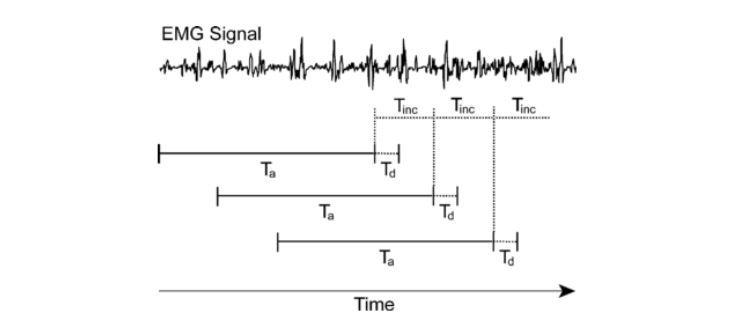
\includegraphics[width=0.92\linewidth]{EMG_Signal}
	\caption{EMG Signal with overlapping windows \cite{englehart2003}.}
	\label{fig:emg_overlap}
\end{figure}

For the neural networks, the gestures were encoded in one-hot format such that a softmax activation function could be used for the output layer. The SVM left the target classes in their numerical form 0 through 3. The data was randomly split 60/20/20 into training, validation, and testing data. The networks were tuned using the validation and testing data, and then after the network parameters were finalized, it was tested with the test data for comparison amongst the three types of networks created. 

\subsection{Feature Extraction}
After the data is windowed, several features are computed for each windowed section to increase the total number of attributes and obtain additional information from the EMG data. There are many options for the time-domain features that can be obtained, but the four most popular options were selected. Each feature is computed for each of the 8 data sensors, resulting in a total of 56 attributes.

\paragraph{Mean Absolute Value (MAV)} 
To compute the MAV, the absolute values are taken for each reading, then averaged across each window, as illustrated in \cref{eqn:mav}, where $(x_n(i))$ is the reading for channel n at time i, and m is the window size.

\begin{equation}
MAV(n) = \frac{1}{m}\sum_{i=1}^{m}\left|(x_n(i)\right|.
\label{eqn:mav}
\end{equation}

\paragraph{Waveform Length (WL)} 
This feature states the cumulative length of the signal, as per \cref{eqn:wl}, where N is the length of the signal and x(i) is the ith sample of the signal.
\begin{equation}
WL = \sum_{i=1}^{N-1}\left|(x(i+1) - x(i)\right|.
\label{eqn:wl}
\end{equation}

\paragraph{Zero Crossing (ZC)}
This feature counts the number of times the signal crosses a predefined threshold $th$ as follows:
\begin{equation}
ZC=\sum_{i=1}^{N-1}f\left[x\left(i\right),x\left(i+1\right)\right],
\label{eqn:zc}
\end{equation}

\noindent where $f(x,y)$ is defined as:

\begin{equation}
f(x,y)=\begin{cases}
1\qquad\text{if}(x\cdot{y})< 0\cap\left|x-y\right|\geq th\\
0\qquad\text{otherwise}
\end{cases}
\label{eqn:zc2}
\end{equation}

\paragraph{Auto-Regressive Coefficients (AR)}
Each channel is represented by a $4^{th}$ order AR model and the features are the coefficients for the model. The coefficients can be computed using \cref{eqn:ar}, where $P$ is the AR order, $ap$ are the AR coefficients, and $w_i$ is a white noise term.
\begin{equation}
 x_i = \sum_{p=1}^{P}a_px_{i-p}+w_i.
\label{eqn:ar}
\end{equation}

\subsection{SVM}
A Support Vector Classifier (SVC) was used to approximate the decision boundaries between the four gesture classes. Four hyperparameters were tuned during training. An L2 regularization parameter $C$ was introduced to prevent the model from overfitting. A kernel parameter specified which kernel to use during computation and offered a variety of paths the model could take towards finding suitable decision boundaries. For instance, the linear kernel would only be effective at finding linearly separable decision boundaries whereas the polynomial and RBF kernels are especially useful when the data points are not linearly separable. When the polynomial kernel function is used, the degree of the polynomial is specified by the 'degree' hyperparameter. Similarly, the 'gamma' parameter specifies the kernel coefficients for the RBF, polynomial and sigmoid functions. The values of the hyperparameters space are given in \Cref{table:svm_param}.

\begingroup
\def\arraystretch{1.2}% row spacing
\setlength{\tabcolsep}{2pt} % column spacing
\begin{table}[b]
	\centering
	\caption{SVM Hyperparameter Tuning Space.}
	\label{table:svm_param}
	\adjustbox{max width=\columnwidth}{
		\begin{tabular}{|l|l|}
			\hline
			\multicolumn{1}{|c|}{\textbf{Hyperparameter}} & \multicolumn{1}{c|}{\textbf{Options}} \\ \hline
			C              & 1, 10, 100, 1000                  \\ \hline
			Kernel         & 'Linear', 'Poly', 'RBF', Sigmoid' \\ \hline
			Degree         & 1, 3, 5, 7                        \\ \hline
			Gamma          & 'Scale', 'Auto'                   \\ \hline
		\end{tabular}}
\end{table}%
\endgroup

A baseline SVC model was instantiated with the default parameters \{‘C’: 1, 'kernel': linear, 'gamma': 'scale'\} which was then fit on the training data. 10-fold cross validation was used to obtain a baseline train score. GridSearchCV was applied to search over the hyperparameter space given in the table above. GridSearchCV exhausted all possible combinations of parameters looking for the model yielding the best 10-fold cross validation accuracy score. Once obtained, the selected model was evaluated on the test set for final results.

\subsection{FFNN}
A simple fully connected FFNN was created to distinguish the gestures from each other. The input layer had 56 neurons as there are 56 features being input into the network, and the output layer had four neurons to support the softmax activation function for the last layer. L2 regularization was used in all layers to help prevent overfitting. The number of hidden layers and the number of neurons in the hidden layer were tuned using the default parameters for the all other hyperparameters. The loss functions of these networks were observed to determine the number of epochs that should be used for fine tuning the network. The range of neurons in the hidden layer ($N_{HL}$) were computed using \cref{eqn:nn_des}, where $D_{TS}$ is the number of data points in the training set, $N_{IL}$ and $N_{OL}$ are the number of neurons in the input and output layer, respectively, and $a$ is a constant that was varied from 4 to 10 to prevent overfitting \cite{demuth2014}. This resulted in using 4, 6, and 8 neurons in the hidden layers.

\begin{equation}
N_{HL}=\frac{D_{TS}}{a*(N_{IL}+N_{OL})}.
%\textit{\# Neurons in hidden layer} = \frac{\textit{\# Data points in training set}}{a*(\textit{\# Neurons in input layer + \# Layers in output layer})}.
\label{eqn:nn_des}
\end{equation}

After the network structure was settled, the learning rate, learning function, and activation function were tuned in a grid search. \Cref{table:fnn_param} summarizes the options investigated for the hyperparameters that were tuned. Default parameters were used for all other options. The models for tuning were evaluated using the accuracy evaluation metric. After completing the hyperparameter tuning, the best model was evaluated on the test data. 

\begingroup
\def\arraystretch{1.2}% row spacing
\setlength{\tabcolsep}{2pt} % column spacing
\begin{table}[t]
	\centering
	\caption{FFNN Hyperparameter Tuning Space.}
	\label{table:fnn_param}
	\adjustbox{max width=\columnwidth}{
		\begin{tabular}{|l|l|}
			\hline
			\multicolumn{1}{|c|}{\textbf{Hyperparameter}} & \multicolumn{1}{c|}{\textbf{Options}} \\ \hline
			Number of Hidden layers            & 0, 1, 2                         \\ \hline
			Number of Neurons in hidden layers & 4, 6, 8                         \\ \hline
			Learning Function                  & 'Adam', 'SGD'                   \\ \hline
			Learning rate                      & 0.001,0.01,0.05,0.1,0.2,0.3,0.4 \\ \hline
			Activation function                & 'ReLU', 'ELU', 'Sigmoid'        \\ \hline
		\end{tabular}}
\end{table}%
\endgroup

\section{Methodology - Novel (LSTM)}
\subsection{Data Preparation}
EMG data from each gesture was divided into sliding windows of 200 ms and 50 ms overlap. Then, each window was stacked on top of each other horizontally to form a 3D array that was going to be used to train the LSTM network. Each row of the 3D array represented a training sample, whereas each column represented the EMG reading of one of the eight channels/sensors of the Myo Armband. The third dimension of the 3D array represented the lag values of each EMG sensor/channel. After creating a 3D array for each gesture, the rows of this 3D array were randomly shuffled and then were divided into the training set, the cross-validation set, and the testing set, each one having 60\%, 20\%, and 20\%, respectively, of the whole gesture dataset. This procedure was repeated for each of the remaining gesture datasets. Having divided the data into the three sets, the data labels were separated and then, one-hot encoding was used on the data labels in order for them to be classified using a softmax activation function. 

\subsection{LSTM}
LSTM networks have been widely used in sequence problems where there exists a time dependency between data points. They have become popularized for being able to retain information over longer periods of time, a problem that traditional RNNs have struggled with. A baseline LSTM model was constructed with a 50-unit LSTM layer which then passed through a dropout layer, dropping 20\% of the neurons. The remaining neurons were fed into a 100-unit dense layer with the ReLU activation function. In order to output classes, the dense layer was connected to a 4-unit softmax layer which outputted gesture classifications. Tuning took place on the number of hidden dense layers, the number of neurons per hidden layer, the activation function and the dropout rate. The values of the hyperparameter space are given in \Cref{table:lstm_param}.

\begingroup
\def\arraystretch{1.2}% row spacing
\setlength{\tabcolsep}{2pt} % column spacing
\begin{table}[b]
	\centering
	\caption{LSTM Hyperparameter Tuning Space.}
	\label{table:lstm_param}
	\adjustbox{max width=\columnwidth}{
		\begin{tabular}{|l|l|}
			\hline
			\multicolumn{1}{|c|}{\textbf{Hyperparameter}} & \multicolumn{1}{c|}{\textbf{Options}} \\ \hline
			Number of Hidden layers            & 0, 1, 2                            \\ \hline
			Number of Neurons in hidden layers & 4, 6, 8                            \\ \hline
			Activation function                & 'ReLU', 'ELU', 'Sigmoid'           \\ \hline
			Dropout rate                       & 0.15, 0.18, 0.21, 0.24, 0.27, 0.30 \\ \hline
	\end{tabular}}
\end{table}%
\endgroup

A baseline LSTM model was instantiated with the parameters \{‘\# Hidden layers’: 1,  ‘\# Neurons per layer’: 100, ‘Activation function’: ReLU, ‘Dropout rate’: 20\%\} which was then fit on the training data. Hold out cross validation was used to obtain a baseline train score. During tuning, RandomSearch randomly sampled a set of parameters from the available parameters and returned the model yielding the lowest hold out validation score. The selected model was then evaluated on the test set for final results.

\section{Results}
\subsection{Evaluation Metrics}
Three metrics were used to evaluate the performance of our models: accuracy, precision and recall. Accuracy was the most important metric since it represents the proportion of true results among the total number of cases examined. Precision was used to examine the proportion of predicted gestures that were actually correct, for each class. Recall was used to evaluate the proportion of actual gestures that were correctly identified by the models. The equations for how we calculated these metrics are given below.

\begin{equation}
\textrm{Accuracy} = \frac{\textrm{\# Correct predictions}}{\textrm{Total \# predictions}},
\label{eqn:acc}
\end{equation}

\begin{equation}
\textrm{Precision} = \frac{\textrm{True Positives}}{\textrm{True Positives + False Positives}} \textrm{, per gesture},
\label{eqn:pr}
\end{equation}

\begin{equation}
\textrm{Recall} = \frac{\textrm{True Positives}}{\textrm{True Positives + False Negatives}} \textrm{, per gesture}.
\label{eqn:rec}
\end{equation}

\subsection{SVM Results}
Results after iterating through the hyperparameter space showed that linear and low-order polynomial models performed the best. In general, linear kernels consistently outperformed all other kernels. Almost every single linear kernel, regardless of the state of other hyperparameters, scored an impressive 99.48\% accuracy on the validation set. This was only 0.4\% lower than the highest score, which was found by a 1st-order polynomial kernel with minimal smoothing. Kernels that performed notably worse were the sigmoid and RBF kernels, scoring up to 75\% worse than their peers when all other hyperparameter values were left equal. Regularization appeared to have minimal effect over the polynomial kernels and no effect on linear kernels. The validation score decreased as the degree of the polynomial kernel increased, signalling the data had a strong preference for linear models. The best performing models and their hyperparameters are summarized in \Cref{table:svm_tun}. The scores reported are their validation scores. Based on these results, Network 1 was selected to be evaluated on the test set. It scored a test accuracy of 99.36\%. \cref{fig:svm_cm} shows the confusion matrix generated the predictions made on the test set by Network 1, and \cref{fig:svm_pr} shows the corresponding precision and recall scores.

\begingroup
\def\arraystretch{1.2}% row spacing
\setlength{\tabcolsep}{2pt} % column spacing
\begin{table}[b]
	\centering
	\caption{SVM Hyptertuning Results.}
	\label{table:svm_tun}
	\adjustbox{max width=\columnwidth}{
		\begin{tabular}{|l|l|l|l|l|l|}
			\hline
			\multicolumn{1}{|c|}{\textbf{Hyperparameter}} & \multicolumn{1}{c|}{\textbf{Network 1}} & Network 2               & Network 3               & Network 4               & Network 5               \\ \hline
			C                                             & 10                                      & 1                       & 1                       & 1                       & 10                      \\ \hline
			Kernel                                        & Polynomial                              & Linear                  & Linear                  & Linear                  & Linear                  \\ \hline
			Degree                                        & 1                                       & 1                       & 3                       & 3                       & 1                       \\ \hline
			Gamma                                         & Scale                                   & Scale                   & Scale                   & Auto                    & Scale                   \\ \hline
			\textit{\textbf{Validation Accuracy}}         & \textit{\textbf{99.52\%}}                 & \textit{\textbf{99.48\%}} & \textit{\textbf{99.48\%}} & \textit{\textbf{99.48\%}} & \textit{\textbf{99.48\%}} \\ \hline
		\end{tabular}}
\end{table}%
\endgroup

\begin{figure}[t]
	\centering
	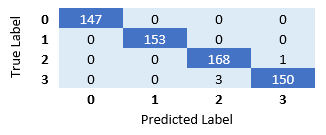
\includegraphics[width=0.88\linewidth]{SVM_confusion_matrix}
	\caption{SVM Confusion Matrix}
	\label{fig:svm_cm}
\end{figure}

\begin{figure}[t]
	\centering
	\includegraphics[width=0.46\linewidth]{SVM_prec_rec}
	\caption{SVM Precision and Recall Scores}
	\label{fig:svm_pr}
\end{figure}

\subsection{FFNN Results}
Upon investigating which network architecture performed best, the 2-layer network consistently resulted in higher accuracies than the 3- and 4-layer networks, as overfitting was beginning to occur. It was found that the loss function stabilized after approximately 30 epochs, thus 120 epochs were used for all further tuning. The 4-layer networks got “stuck” and would not pass accuracies of 25-35\%, despite trying multiple learning rates and 200+ epochs. The grid search was performed with the 2 layer network and the best performing 3 layer network (4 neurons in the hidden layer) to determine if tuning would improve the performance of the 3 layer network. The best performing models and their hyperparameters are summarized in \Cref{table:fnn_tun}. Again, it was found that the 2-layer network consistently performed better than the 3-layer one. When the SGD learning function was used, there was no dependency for the model’s accuracy on the learning rate once it was larger than 0.05. On the other hand, with the Adam learning function, the accuracy decreased as the learning rate increased. Additionally, the Adam learning function frequently resulted in a loss function that oscillated about an asymptote, as opposed to converging to the asymptote like the SGD function did. For both learning functions, the number of epoch required for the loss function to reach the asymptote decreased as the learning rate increased. The sigmoid activation function resulted in accuracies around 97-98\%, whereas 99\% accuracy was achieved with both ReLU and ELU activation functions. Overall, Network 1 showed the most promise, scoring an accuracy of 99.36\% on the validation set and an accuracy of 98.71\% on the test set. \cref{fig:fnn_cm} displays the confusion matrix for Network 1 on the test data, while \cref{fig:fnn_pr} shows the corresponding precision and recall values for each gesture. The rows are what the gesture is, whereas the columns are what the FFNN predicted. The network was capable of identifying gesture 1 with no problems. It struggled more with gestures 3 and 4. Gesture 3 was sometimes mistaken for 2 or 4, whereas gesture 4 was mistaken for all the other options in 1-2 instances.

\begingroup
\def\arraystretch{1.2}% row spacing
\setlength{\tabcolsep}{2pt} % column spacing
\begin{table}[t]
	\centering
	\caption{FNN Hyptertuning Results.}
	\label{table:fnn_tun}
	\adjustbox{max width=\columnwidth}{
		\begin{tabular}{|l|l|l|l|l|l|}
			\hline
			\multicolumn{1}{|c|}{\textbf{Hyperparameter}} & \multicolumn{1}{c|}{\textbf{Network 1}} & Network 2               & Network 3               & Network 4               & Network 5               \\ \hline
			\# Hidden layers                       & 2                                       & 2                       & 2                       & 2                       & 3                       \\ \hline
			\# Neurons in hidden layers            & -                                       & -                       & -                       & -                       & 4                       \\ \hline
			Learning Function                             & Sgd                                     & Adam                    & Sgd                     & Sgd                     & Sgd                     \\ \hline
			Learning rate                                 & 0.05-0.4                                & 0.001                   & 0.05-0.4                & 0.05-0.4                & 0.05-0.4                \\ \hline
			Activation function                           & ReLU                                    & ELU                     & ELU                     & Sigmoid                 & Sigmoid                 \\ \hline
			\textit{\textbf{Validation Accuracy}}         & \textit{\textbf{99.36}}                 & \textit{\textbf{99.36}} & \textit{\textbf{99.20}} & \textit{\textbf{98.71}} & \textit{\textbf{98.87}} \\ \hline
		\end{tabular}}
\end{table}%
\endgroup

\begin{figure}[t]
	\centering
	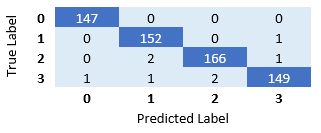
\includegraphics[width=0.88\linewidth]{FFNN_confusion_matrix}
	\caption{FNN Confusion Matrix}
	\label{fig:fnn_cm}
\end{figure}

\begin{figure}[!t]
	\centering
	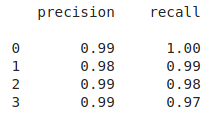
\includegraphics[width=0.46\linewidth]{FFNN_prec_rec}
	\caption{FNN Precision and Recall Scores}
	\label{fig:fnn_pr}
\end{figure}

\subsection{LSTM Results}
After reviewing the results from the RandomSearch hyperparameter tuning process, we found that networks with 3 to 4 hidden layers were consistently preferred, although one shallow network with a single hidden layer performed substantially well. We observed no strong preference for the number of neurons per hidden layer, though it’s worth noting that the highest scoring models tended to have a couple dense layers of 100+ neurons. We also found that having too harsh of a dropout policy negatively affected the models performance. Results show that a dropout rate of 18\%-24\% generated the highest validation scores, with scores dipping drastically after the 27\% mark. Finally, we found that the ELU activation function consistently outperformed the ReLU function and was the activation function of choice for the first 8 out of 10 top models returned by RandomSearch. The best performing models and their hyperparameters are summarized in \Cref{table:lstm_tun}. The scores reported are their validation scores. Network 1 was evaluated on the test set and scored a test accuracy of 99.36\%. \cref{fig:lstm_a_l} shows the training accuracy and loss graphs for Network 1, which was selected from RandomSearch. \cref{fig:lstm_cm} shows the confusion matrix for Network 1 on the test set, , while \cref{fig:lstm_pr} shows the corresponding precision and recall values for each gesture. 

\begingroup
\def\arraystretch{1.2}% row spacing
\setlength{\tabcolsep}{2pt} % column spacing
\begin{table}[b]
	\centering
	\caption{LSTM Hyptertuning Results.}
	\label{table:lstm_tun}
	\adjustbox{max width=\columnwidth}{
		\begin{tabular}{|l|l|l|l|l|l|}
			\hline
			\multicolumn{1}{|c|}{\textbf{Hyperparameter}} & \multicolumn{1}{c|}{\textbf{Network 1}} & Network 2               & Network 3               & Network 4               & Network 5               \\ \hline
			\# Hidden layers                       & 3                                       & 1                       & 3                       & 4                       & 3                       \\ \hline
			\# Neurons in hidden layers            & 50, 200, 200                            & 50                      & 100, 50, 100            & 100, 50, 150, 150       & 150, 150, 200           \\ \hline
			Activation function                           & ELU                                     & ELU                     & ELU                     & ELU                     & ELU                     \\ \hline
			Dropout rate                                  & 21\%                                    & 24\%                    & 15\%                    & 21\%                    & 18\%                    \\ \hline
			\textit{\textbf{Validation Accuracy}}         & \textit{\textbf{99.68}}                 & \textit{\textbf{99.67}} & \textit{\textbf{99.64}} & \textit{\textbf{99.61}} & \textit{\textbf{99.56}} \\ \hline
		\end{tabular}}
\end{table}%
\endgroup

\begin{figure}[t]
	\centering
	\begin{subfigure}[b]{0.92\linewidth}
		\centering
		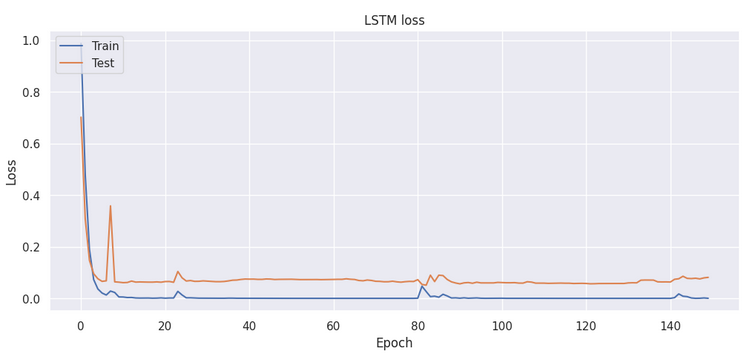
\includegraphics[width=0.92\linewidth]{LSTM_train_loss}
		\caption{}
		\label{fig:lstm_loss}
	\end{subfigure}
%	\hfill
	\begin{subfigure}[b]{0.92\linewidth}
		\centering
		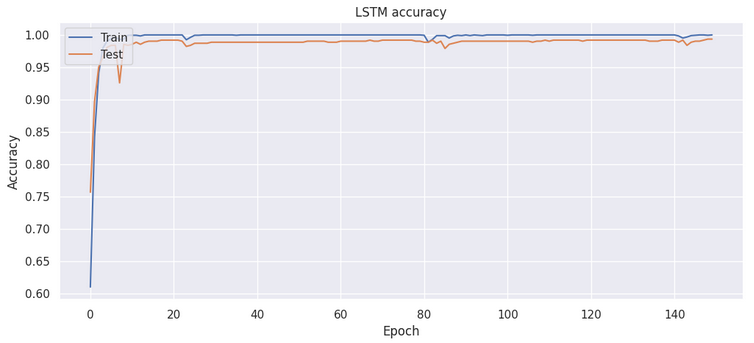
\includegraphics[width=0.92\linewidth]{LSTM_train_accuracy}
		\caption{}
		\label{fig:lstm_acc}
	\end{subfigure}
	\caption{LSTM accuracy and training loss for Network 1. a) LSTM Training Loss. b) LSTM Training Accuracy.}
	\label{fig:lstm_a_l}
\end{figure}

%\begin{figure}[t]
%	\centering
%	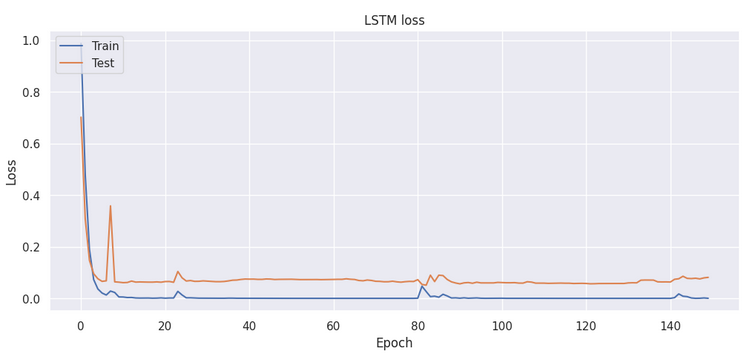
\includegraphics[width=0.92\linewidth]{LSTM_train_loss}
%	\caption{LSTM Training Loss}
%	\label{fig:lstm_loss}
%\end{figure}

%\begin{figure}[t]
%	\centering
%	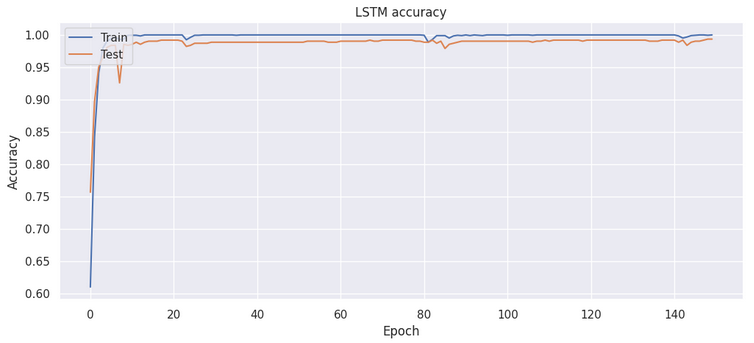
\includegraphics[width=0.92\linewidth]{LSTM_train_accuracy}
%	\caption{LSTM Training Accuracy}
%	\label{fig:lstm_acc}
%\end{figure}

\begin{figure}[t]
	\centering
	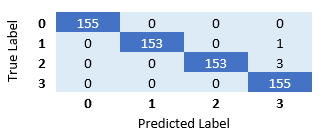
\includegraphics[width=0.88\linewidth]{LSTM_confusion_matrix}
	\caption{LSTM Confusion Matrix}
	\label{fig:lstm_cm}
\end{figure}

\begin{figure}[!t]
	\centering
	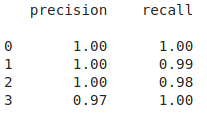
\includegraphics[width=0.46\linewidth]{LSTM_prec_rec}
	\caption{LSTM Precision and Recall Scores}
	\label{fig:lstm_pr}
\end{figure}

\begingroup
\def\arraystretch{1.2}% row spacing
\setlength{\tabcolsep}{2pt} % column spacing
\begin{table}[b]
	\centering
	\caption{Final Model Comparison.}
	\label{table:final_comp}
	\adjustbox{max width=\columnwidth}{
		\begin{tabular}{|l|l|l|l|}
			\hline
			Method                          & SVM                     & FFNN                    & LSTM                    \\ \hline
			\textit{\textbf{Test Accuracy}} & \textit{\textbf{99.36}} & \textit{\textbf{98.71}} & \textit{\textbf{99.68}} \\ \hline
	\end{tabular}}
\end{table}%
\endgroup

\subsection{Model Comparison}
\Cref{table:final_comp} summarizes the test accuracy for the three methods. It is clear that all three methods are very successful. Based on the tuning that was performed, the SVM and LSTM networks performed better than the FFNN. While care was taken to tune each network approximately the same amount, it is possible that with further tuning the FFNN could achieve the accuracy obtained by the other two methods. From observing the precision and recall tables, it can be seen that each architecture had issues with different gestures. The novel LSTM neural network mis-identified gesture 2 more than others. It had no issues with gestures 0 or 3. Conversely, the SVM and FFNN had more issues with gesture 3 than the others. This difference could be due to the feature extraction that was performed for the FFNN and the SVM. It is fortunate to know that the LSTM network, once trained, performs comparably to the standard methods. This is advantageous for real-time systems (such as video games for rehabilitation), as they would not have to take the time or computational power to compute all the features while the system is running, which could lead to faster response times.









\bibliographystyle{IEEEtran}
%\IEEEtriggeratref{24}
\bibliography{References/references}




% that's all folks
\end{document}


